\documentclass[a4j]{jsarticle}
\usepackage{graphicx}
\usepackage{listings}

\title{2024年度プログラミング\textsc{iii} 第1回レポート}
\author{学籍番号: 35714121 \\ 氏名: 福富隆大}
\date{2024年10月4日}
\usepackage{graphicx}

\begin{document}
\maketitle

\textbf{1 はじめに}

本レポートは演習課題1の実行結果をまとめたものである。

\textbf{2 演習課題}

\textmd{2.1 課題1}

課題の実行結果を図1に示す。

\begin{figure}[htbp]
  \centering
  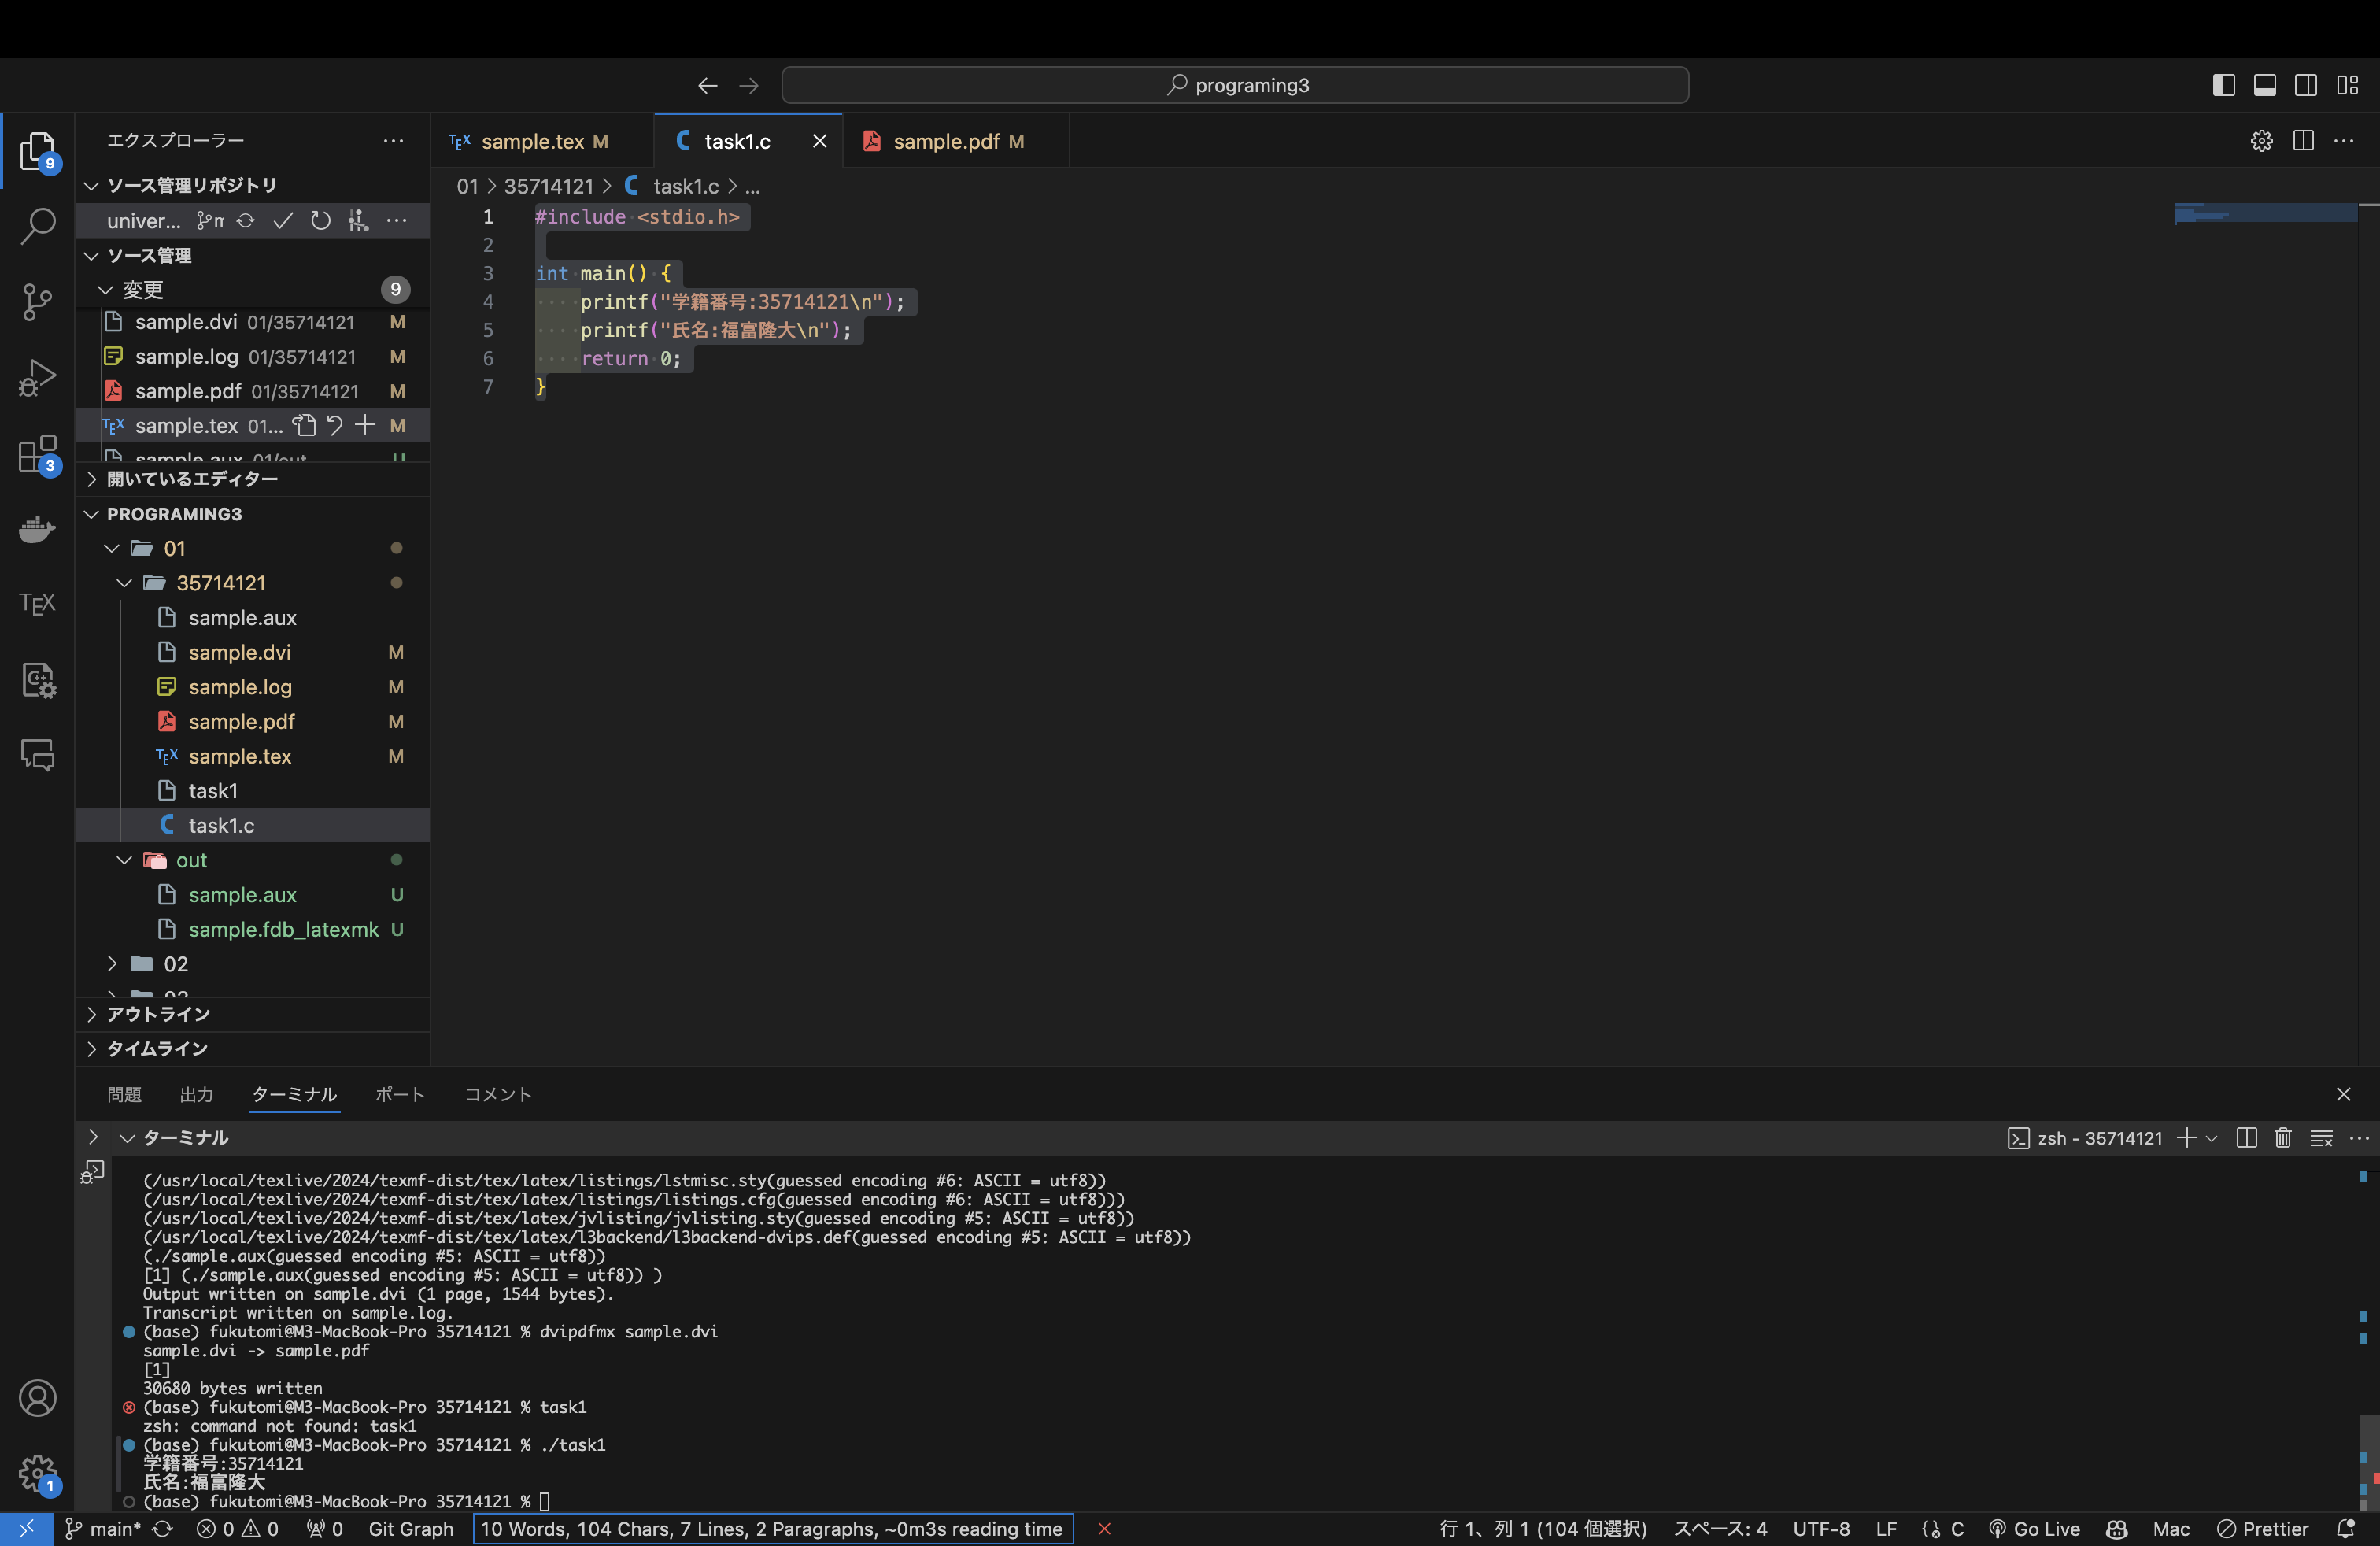
\includegraphics[width=10cm]{task1.eps}
  \caption{(画面下のターミナルの部分に実行結果があります)}
  \label{fig:sample}
\end{figure}

\textbf{3 ソースコード}

\begin{lstlisting}[language=Python, basicstyle=\ttfamily\small, frame=single]
  #include <stdio.h>

  int main() {
      printf("学籍番号:35714121\n");
      printf("氏名:福富隆大\n");
      return 0;
  }
\end{lstlisting}

\end{document}
